\chapter{Προβλέψεις Διακλαδώσεων με Σφάλματα}
\label{chap4}

\section{Εισαγωγή}
\label{chap4_Intro}

Όπως έχει αποδειχθεί από πληθώρα ερευνητικών εργασιών, τα στοιχεία μνήμης είναι επιρρεπή σε βλάβες όταν η τάση λειτουργίας που εφαρμόζεται σε αυτές είναι πολύ-χαμηλού επιπέδου. Βασική αιτία είναι η χρήση μικρού μεγέθους κυψελίδων (συνήθως \en{6T SRAM}), ώστε να καταλαμβάνουν όσο το δυνατόν μικρότερο εμβαδόν.
\par
Η Μονάδα Δυναμικής Πρόβλεψης Διακλαδώσεων αποτελείται από ένα σύνολο κυψελίδων μνήμης και επομένως αναμένεται ορισμένα από αυτά να μην λειτουργούν σωστά όταν η τάση λειτουργίας μειώνεται, προκαλώντας έτσι μείωση στην απόδοσης του συστήματος. Σύμφωνα με τη λειτουργία της μονάδας, όπως παρουσιάστηκε στην Ενότητα \ref{chap2_DynamicBranchPredictionUnit}, η ορθή εκτέλεση ενός προγράμματος δεν θα επηρεαστεί καθώς η Μονάδα Δυναμικής Πρόβλεψης Διακλαδώσεων παρέχει απλώς μία πρόβλεψη, η οποία στη χειρότερη περίπτωση θα είναι λανθασμένη και σε μελλοντικό χρόνο θα ανιχνευθεί. Συνεπώς η διόρθωσή τους δεν κρίνεται απαραίτητη. Στο παρόν κεφάλαιο μελετάται η επιβάρυνση που πιθανός θα προκαλέσουν τα σφάλματα αυτά στη συνολική απόδοση του συστήματος, και συνεπώς στην κατανάλωσή του. Ο υπολογισμός της μείωσης της απόδοσης, δηλαδή του ρυθμού ολοκλήρωσης εντολών (\ipc), εξαιτίας της ύπαρξης σφαλμάτων υπολογίζεται ώς:

\begin{equation}
    \label{eqn:chap4_IPCfaulty}
    \mathgr{Μείωση}\_IPC = \frac{IPC_\mathgr{χωρίς\_σφάλματα} - IPC_\mathgr{με\_σφάλματα}}{IPC_\mathgr{χωρίς\_σφάλματα}}
\end{equation}

Τα αποτελέσματα που παρουσιάζονται εξήχθησαν από τον εξομοιούμενο \en{x86} επεξεργαστή για διαφορετικές παραμετροποιήσεις του. Αναλυτικές πληροφορίες για το βασικό μοντέλο επεξεργαστή καθώς και για τη διαδικασία εξομοίωσης περικλείονται στα Κεφάλαια \ref{chap6} και \ref{chap7} αντίστοιχα.

%----------------------------------------------------------%

\section{Σφάλματα στη Μονάδα Δυναμικής Πρόβλεψης Διακλαδώσεων}
\label{chap4_DynamicBranchPredictionUnitFaults}

Σύμφωνα με την έως τώρα ανάλυση, η πολύ μεγάλη μείωση της τάσης λειτουργίας αναμένεται να έχει επιπτώσεις στη Μονάδα Δυναμικής Πρόβλεψης Διακλαδώσεων, προκαλώντας την αύξηση του χρόνου ολοκλήρωσης των προγραμμάτων. Οι μελέτες \cite{hsieh2009tolerance} και \cite{hardy2012performance} επικεντρώνεται στα σφάλματα μόνιμης τιμής μίας μονάδα πρόβλεψης τύπου \en{gshare}. Επίσης, στην \cite{foutris2013ssing} αναλύονται τα σφάλματα μόνιμης τιμής στα στοιχεία που χρησιμοποιούνται αποκλειστικά για την ενίσχυση της απόδοσης, όπως είναι και η μονάδα πρόβλεψης τύπου \en{bimodal} που χρησιμοποιείται. Αντιθέτως, η συγκεκριμένη μελέτη επικεντρώνεται στην εμφάνιση τόσο μόνιμων όσο και προσωρινών σφαλμάτων σε μία μονάδα πρόβλεψης επιλεκτικής διάταξης (\en{tournament}).
\par
Για τη μοντελοποίηση των ελαττωματικών κυψελίδων μνήμης ώς σφάλματα στη Μονάδας Δυναμικής Πρόβλεψης Διακλαδώσεων, παρήχθησαν χάρτες σφαλμάτων για κάθε πιθανότητα σφάλματος στην αντίστοιχη τάση λειτουργίας. Τα σφάλματα θεωρούνται ομοιόμορφα κατανεμημένα στις κυψελίδες της μνήμης και ξεκινώντας από τη μηδενική πιθανότητα σφάλματος (ονομαστική τάση λειτουργίας), σταδιακά αυξάνεται (μείωση της τάσης λειτουργίας) εισάγοντας τα αντίστοιχα πρόσθετα σφάλματα. Επομένως, ο χάρτης σφαλμάτων για την πιθανότητα σφάλματος $2N$ θα περιέχει τα σφάλματα του χάρτη της πιθανότητας σφάλματος $N$ καθώς και κάποια επιπλέον ώστε τα συνολικά σφάλματα να είναι διπλάσια, όπως φαίνεται και από το παράδειγμα του Σχήματος \ref{fig:chap4_fmap_creation}.

\begin{figure}[ht]
    \centering
    \fbox{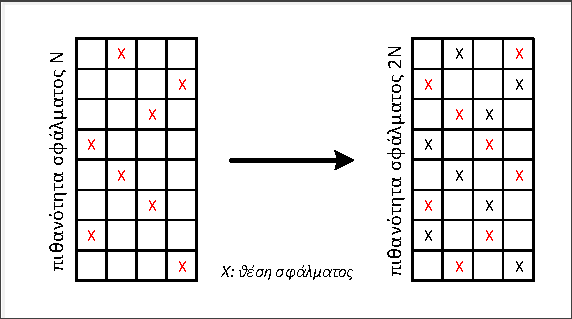
\includegraphics[trim=0.7cm 0.6cm 0.5cm 0.6cm, clip=true]{\hardwareDIR/chap4_fault_maps.pdf}}
    \caption{Δημιουργία χάρτη σφαλμάτων διπλάσιας πιθανότητας σφάλματος}
    \label{fig:chap4_fmap_creation}
\end{figure}

Το συνολικό πλήθος σφαλμάτων που θα περιέχει ένας χάρτης σε κάθε περίπτωση υπολογίζεται από την ακόλουθη σχέση:
\begin{equation}
    \textit{Πλήθος Σφαλμάτων} = \textit{Πιθανότητα Σφάλματος} \times \textit{Πλήθος Κυψελίδων Μνήμης}
\end{equation}

Σύμφωνα με τη μελέτη του \en{Sanchez} και άλλων \cite{sanchez2011analytical}, για την πραγματοποίηση μεγαλύτερης ακρίβειας μετρήσεων οι οποίες βασίζονται σε χάρτες σφαλμάτων πρέπει να εξεταστούν από 100 έως 1000 διαφορετικοί χάρτες. Ο λόγος που απαιτείται αυτός ο μεγάλος αριθμός διαφορετικών χαρτών είναι η ανομοιογένεια των προσπελάσεων στα σύνολα της μνήμης μεταξύ των μετροπρογραμμάτων. Επομένως πραγματοποιήθηκαν 100 επαναλήψεις της διαδικασίας παραγωγής χαρτών σφαλμάτων, για διαφορετικές πιθανότητες. Το πλήθος αυτό θεωρείται ικανοποιητικό για την εξαγωγή συμπερασμάτων στη συγκεκριμένη δομή.
\par
Στις ακόλουθες υποενότητες παρουσιάζονται οι αντιστοιχίες μεταξύ πιθανότητας σφάλματος και πλήθους σφαλμάτων για τα στοιχεία μνήμης της Μονάδας Δυναμικής Πρόβλεψης Διακλαδώσεων, καθώς και οι επιπτώσεις που έχουν στην απόδοση της Κεντρικής Μονάδας Επεξεργασίας. Το εξομοιούμενο μοντέλο είναι αυτό του Πίνακα \ref{tab:chap6_gem5parameters} που παρουσιάζεται στο Κεφάλαιο \ref{chap6}, και το οποίο χρησιμοποιείται στην πλειοψηφία των περιπτώσεων.

%----------------------------------------------------------%

\subsection{Σφάλματα στον Πίνακα Πρόβλεψης Διακλάδωσης}
\label{chap4_BranchPredictorFaults}

Στην παρούσα υποενότητα μελετάται η επιρροή που θα έχει η μεγάλη μείωση της τάσης λειτουργίας στην ακρίβεια του Πίνακα Πρόβλεψης Διακλάδωσης. Αρχικά, το Σχήμα \ref{fig:chap4_bpu_fmaps} αναδεικνύει το ποσοστό των θέσεων μνήμης που αποτελούν τον Πίνακα Πρόβλεψης Διακλάδωσης και θα περιέχουν τουλάχιστον ένα σφάλμα. Σε αυτή την περίπτωση θεωρείται πως η θέση μνήμης είναι ελαττωματική καθώς το ιστορικό προβλέψεων που αποθηκεύεται σε αυτή θα δέχεται αλλοίωση από το εσφαλμένο δυαδικό ψηφίο.

\begin{figure}[ht]
    \centering
    \fbox{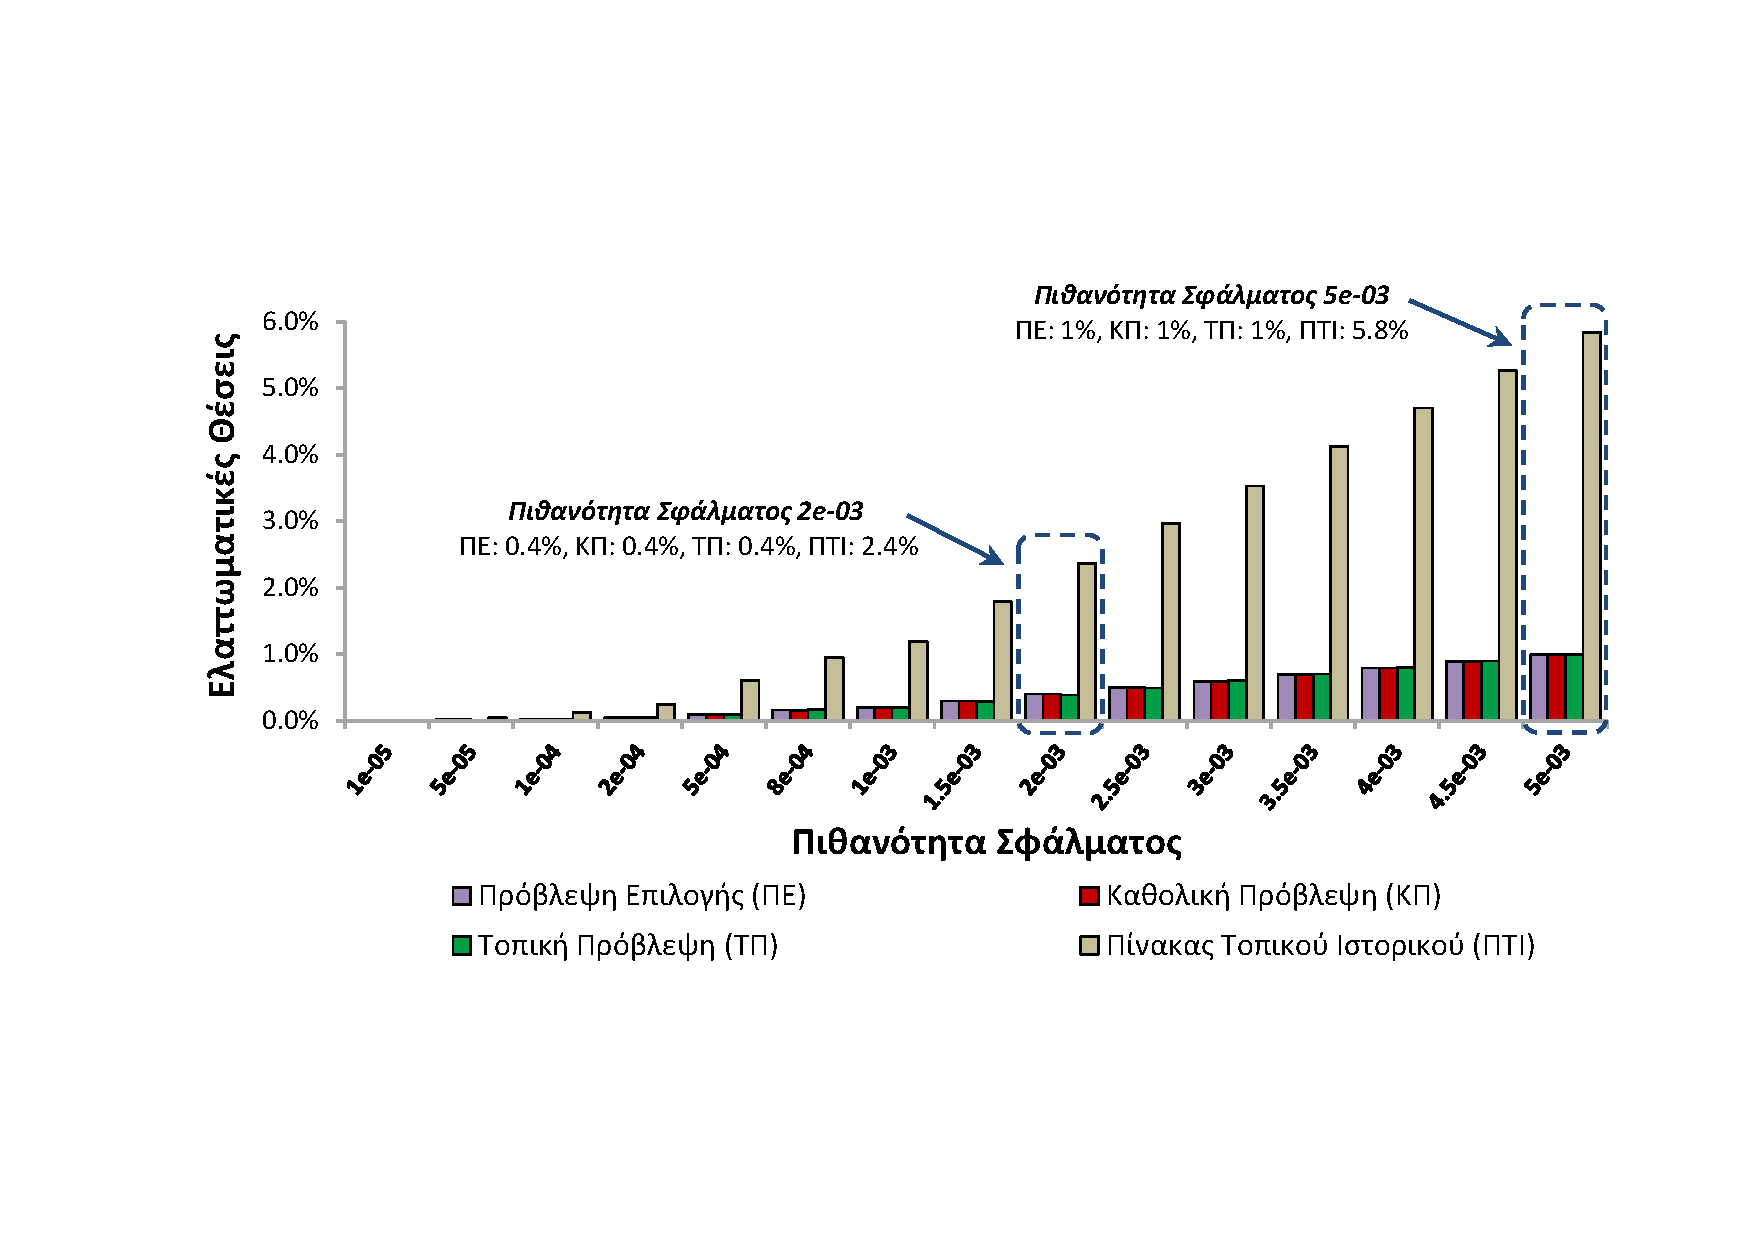
\includegraphics[width=0.9\linewidth, trim=3.4cm 4.7cm 2.2cm 4.8cm, clip=true]{\resultsDIR/chap4_BPU_faulty_entries.pdf}}
    \caption{Σφάλματα στον Πίνακα Πρόβλεψης Διακλάδωσης}
    \label{fig:chap4_bpu_fmaps}
\end{figure}

Όπως φαίνεται και από το γράφημα του Σχήματος \ref{fig:chap4_bpu_fmaps}, εξαιτίας του μικρού μεγέθους των στοιχείων μνήμης το ποσοστό ελαττωματικών θέσεων σε αυτές είναι σχετικά μικρό, ακόμη και σε μεγάλες πιθανότητες σφάλματος. Συγκεκριμένα, το πλήθος κυψελίδων κάθε στοιχείου μνήμης του Πίνακα Πρόβλεψης Διακλάδωσης είναι:

\begin{description} [itemsep=0.5pt]
    \item[Πρόβλεψη Επιλογής(ΠΕ):] 16384 θέσεις $\times$ 2 δ.ψ./θέση = 32768 κυψελίδες
    \item[Καθολική Πρόβλεψη(ΚΠ):] 16384 θέσεις $\times$ 2 δ.ψ./θέση = 32768 κυψελίδες
    \item[Τοπική Πρόβλεψη(ΚΠ):] 4096 θέσεις $\times$ 3 δ.ψ./θέση = 12288 κυψελίδες
    \item[Πίνακας Τοπικού Ιστορικού(ΠΤΙ):] 4096 θέσεις $\times$ 12 δ.ψ./θέση = 49152 κυψελίδες
    \item[Καταχωρητής Καθολικού Ιστορικού(ΚΚΙ):] 12 κυψελίδες
\end{description}

Με βάση τα ποσοστά του Σχήματος \ref{fig:chap4_bpu_fmaps} στη μέγιστη πιθανότητα σφάλματος $\expnum{5}$ στις διατάξεις πρόβλεψης το 1\% των θέσεων περιέχει τουλάχιστον ένα ελαττωματικό δυαδικό ψηφίο, ενώ στον Πίνακα Τοπικού Ιστορικού το ποσοστό αυτό ανέρχεται σε 5.8\%. Συνεπώς, αναμένεται πως οι επιπτώσεις της μείωσης της τάσης λειτουργίας θα είναι ελάχιστες στην επιτυχία του πρώτου επιπέδου πρόβλεψης. Η μείωση της απόδοσης εξαιτίας της ύπαρξης σφαλμάτων στον Πίνακα Πρόβλεψης Διακλάδωσης παρουσιάζεται στο Σχήμα \ref{fig:chap4_bpu_ipc}, όπου κατά μέσο όρο είναι μικρότερη από 1\%.

\begin{figure}[t]
    \centering
    \fbox{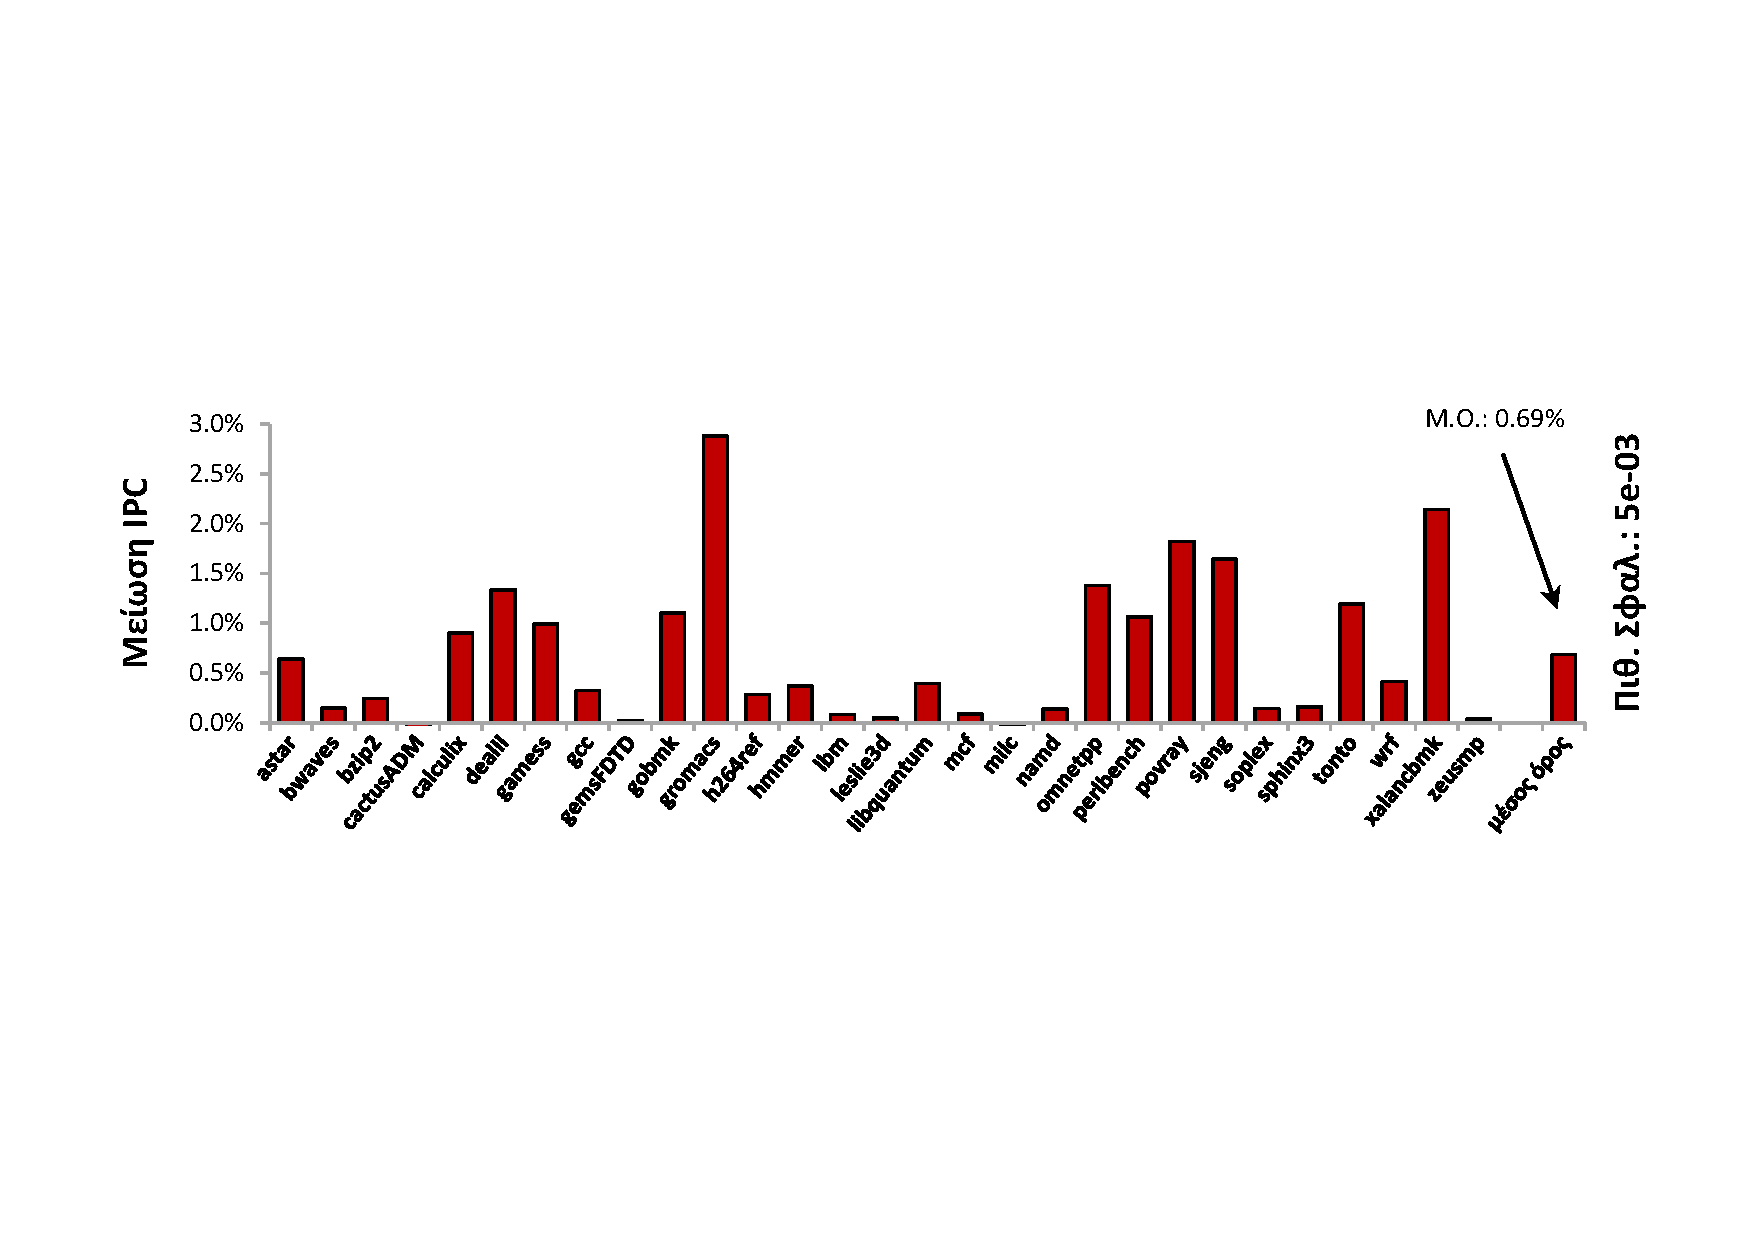
\includegraphics[width=\linewidth, trim=2cm 6.8cm 1.8cm 6.8cm, clip=true]{\resultsDIR/chap4_BPU_faulty_ipc.pdf}}
    \caption{Μείωση του ρυθμού ολοκλήρωσης εντολών εξαιτίας των σφαλμάτων στον Πίνακα Πρόβλεψης Διακλάδωσης, σε σχέση με την περίπτωση εφαρμογής της ονομαστικής τάσης στην ίδια συχνότητα λειτουργίας}
    \label{fig:chap4_bpu_ipc}
\end{figure}

\begin{figure}[!b]
    \centering
    \fbox{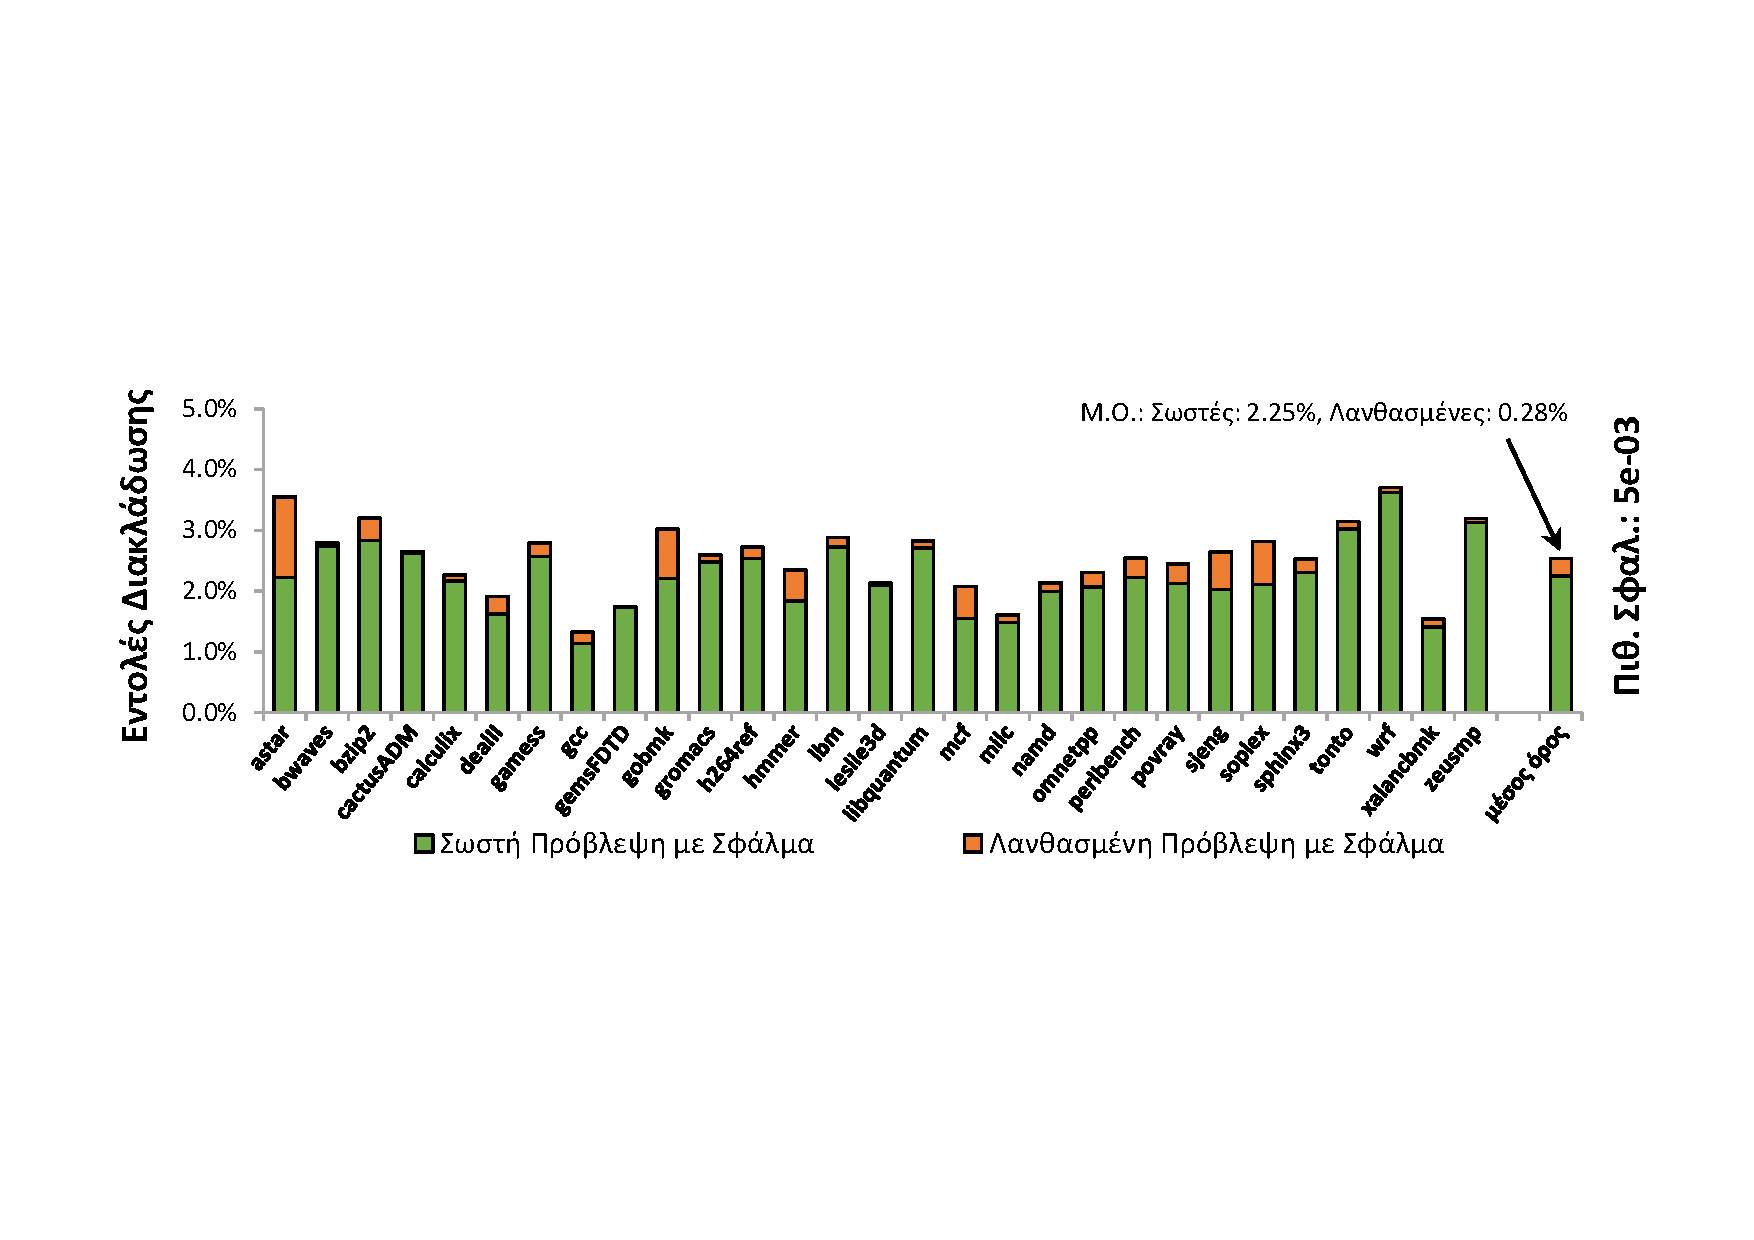
\includegraphics[width=\linewidth, trim=2cm 6.5cm 1.8cm 6.5cm, clip=true]{\resultsDIR/chap4_BPU_faulty_predictions.pdf}}
    \caption{Ποσοστό εκτελούμενων εντολών διακλάδωσης των οποίων η πρόβλεψη περιέχει κάποιο σφάλμα}
    \label{fig:chap4_bpu_branches}
\end{figure}

Για την περαιτέρω μελέτη των επιπτώσεων των σφαλμάτων αυτών, παρουσιάζεται το ποσοστό εντολών διακλάδωσης που εκτελέστηκαν και στις οποίες η εξαγωγή τελικής πρόβλεψης επηρεάστηκε από ελαττωματική θέση μνήμης. Μία τέτοια πρόβλεψη θα περιγράφεται ως πρόβλεψη με σφάλμα. Για παράδειγμα, έστω ότι η θέση που διαβάζεται από την Καθολική Πρόβλεψη περιέχει σφάλμα και η Πρόβλεψη Επιλογής διαλέξει την Καθολική Πρόβλεψη ως πιο έγκυρη, τότε η πρόβλεψη που θα εξαχθεί θα περιέχει σφάλμα. Μία πρόβλεψη με σφάλμα δεν συνεπάγεται πως είναι και λανθασμένη καθώς το σφάλμα μπορεί να προκαλέσει την εξαγωγή σωστής πρόβλεψης, όπως φαίνεται και στο γράφημα του Σχήματος \ref{fig:chap4_bpu_branches}, όπου το άθροισμα των ποσοστών πράσινων και πορτοκαλί αποχρώσεων ισοδυναμεί με το ποσοστό εντολών διακλάδωσης που εκτελέστηκαν και στην πρόβλεψή τους συμμετείχε στοιχείο με σφάλμα (προβλέψεις με σφάλμα), από το σύνολο των εντολών διακλάδωσης που εκτελέστηκαν.
\par
Από τις συνολικές εντολές διακλάδωσης που εκτελέστηκαν, σε μόλις 2.53\% αυτών θα έχουν συμμετάσχει ελαττωματικές κυψελίδες στην εξαγωγή πρόβλεψης. Επίσης, από το ποσοστό αυτό, μόνο στο 0.28\% αποδείχθηκε πως η πρόβλεψη με σφάλμα ήταν ταυτόχρονα και λανθασμένη. Παράδειγμα περίπτωσης όπου ένα σφάλμα μπορεί να μην προκαλέσει καμία μείωση στην ευστοχία αποτελεί η περίπτωση όπου η Πρόβλεψη Επιλογής περιέχει σφάλμα και εξαιτίας αυτού επιλέγεται το αποτέλεσμα της Τοπικής αντί της Καθολικής Πρόβλεψης. Εάν η Τοπική Πρόβλεψη αποδειχθεί σωστή τότε η επίπτωση αυτού του σφάλματος θα είναι μηδενική.
\par
Από τη μελέτη της παρούσας υποενότητας κατέστη σαφές πως η ανάπτυξη κατάλληλης τεχνικής ανοχής σφαλμάτων του Πίνακα Πρόβλεψης Διακλάδωσης δεν είναι απαραίτητη. Για το λόγο αυτό η παρούσα μελέτη επικεντρώνεται στα σφάλματα που εμφανίζονται στον Πίνακα Πρόβλεψης Διακλάδωσης, της οποίας το μέγεθός είναι αρκετά μεγαλύτερο και επομένως αναμένεται να εμφανίσει σημαντικό πλήθος ελαττωματικών στοιχείων.

%----------------------------------------------------------%

\subsection{Σφάλματα στον Πίνακα Πρόβλεψης Προορισμού Διακλάδωσης}
\label{chap4_BranchTargetBufferFaults}

Όπως είναι αναμενόμενο, η μεγάλη μείωση της τάσης λειτουργίας θα επηρεάσει και τη λειτουργία του Πίνακα Πρόβλεψης Προορισμού Διακλάδωσης. Η εμφάνιση σφαλμάτων στον πίνακα θα έχει ως συνέπεια την υποβάθμιση της ακρίβειας πρόβλεψης διευθύνσεων και επομένως της απόδοσης. Για να εξασφαλιστεί πως δεν θα ληφθεί λανθασμένη διεύθυνση εξαιτίας ενός σφάλματος στον Πίνακα Πρόβλεψης Προορισμού Διακλάδωσης, κάτι που μπορεί να επιφέρει σημαντική αύξηση του χρόνου εκτέλεσης του προγράμματος, τα πλαίσια που περιέχουν τουλάχιστον μία ελαττωματική κυψελίδα απενεργοποιούνται χρησιμοποιώντας την τεχνική απενεργοποίησης πλαισίου, η οποία εφαρμόζεται συχνά στην Κρυφής Μνήμη πρώτου επιπέδου όπως αναφέρθηκε στην Ενότητα \ref{chap3_FaultTaulerance}. Για την υλοποίηση αυτής της τεχνικής αρκεί η προσθήκη ενός δυαδικού ψηφίου ανά θέση μνήμης, το αποκαλούμενο ως $``$Ψηφίο Σφάλματος$"$, το οποίο δηλώνει εάν ανιχνεύτηκε ελαττωματική κυψελίδα στην αντίστοιχη θέση κατά τη διαδικασία του ελέγχου.
\par
Στην παρούσα υποενότητα μελετάται η επιρροή που θα έχει η μείωση του έγκυρου χώρου αποθήκευσης του Πίνακα Πρόβλεψης Προορισμού Διακλάδωσης (ΠΠΠΔ), το ποσοστό του οποίου παρουσιάζεται στο Σχήμα \ref{fig:chap4_btb_fmaps}.

\begin{figure}[!t]
    \centering
    \fbox{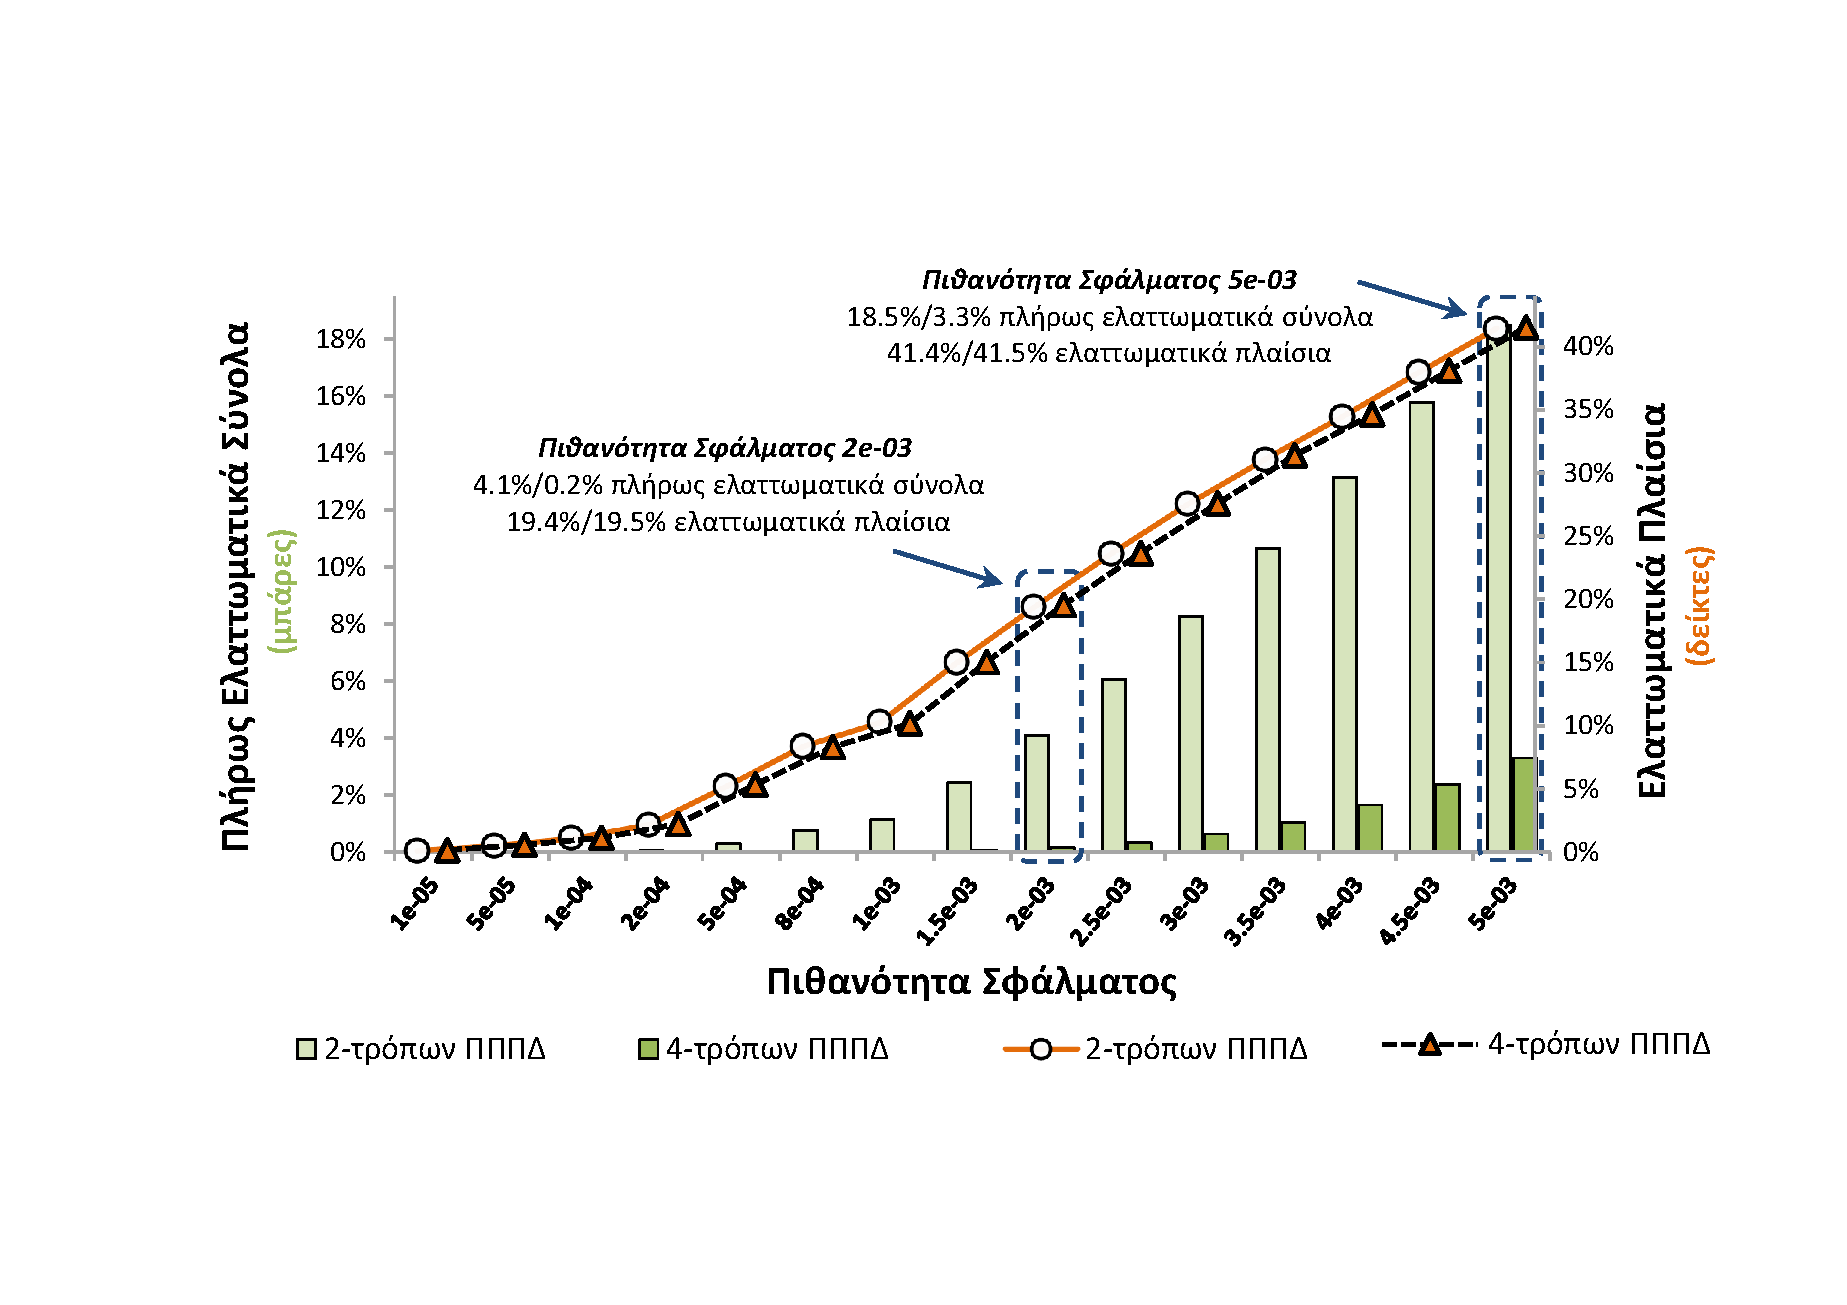
\includegraphics[width=0.9\linewidth, trim=3.5cm 4cm 2cm 4.3cm, clip=true]{\resultsDIR/chap4_BTB_faulty_entries_and_sets.pdf}}
    \caption{Σφάλματα στον Πίνακα Πρόβλεψης Προορισμού Διακλάδωσης (ΠΠΠΔ)}
    \label{fig:chap4_btb_fmaps}
\end{figure}

Το γράφημα του Σχήματος \ref{fig:chap4_btb_fmaps} αποτελείται από δύο κατηγορίες δεδομένων. Οι μπάρες πράσινων αποχρώσεων παριστάνουν το ποσοστό των πλήρως ελαττωματικών συνόλων, δηλαδή τα σύνολα που όλα τα πλαίσια περιέχουν τουλάχιστον μία ελαττωματική κυψελίδα (κάθετος άξονας αριστερά). Το χαρακτηριστικό αυτών των θέσεων είναι η αδυναμία αποθήκευσης πληροφορίας για ένα πλήθος εντολών διακλάδωσης. Το δεύτερο δεδομένο, το οποίο αναπαρίσταται στο γράφημα με τη μορφή δεικτών στις νοητές καμπύλες πορτοκαλί και μαύρων αποχρώσεων, εκφράζουν το αντίστοιχο ποσοστό των ελαττωματικών πλαισίων για κάθε πιθανότητα σφάλματος (κάθετος άξονας δεξιά). Τα σχετικά μικρού μεγέθους πλαίσια, τα οποία αποτελούνται από τα πεδία ετικέτας, διεύθυνσης προορισμού και ορισμένες ακόμα πληροφορίες, συνεπάγονται τη σχετικά μικρή πιθανότητα μίας θέσης να είναι ελαττωματική, συγκριτικά με μία θέση Κρυφής Μνήμης (λιγότερα δυαδικά ψηφία ανά πλαίσιο συνεπάγεται και μικρότερη πιθανότητα να είναι ελαττωματικό). Το γράφημα του Σχήματος \ref{fig:chap4_btb_fmaps} εκφράζει το μέσο όρο 100 χαρτών σφαλμάτων για κάθε πιθανότητα σφάλματος.
\par
Τα δεδομένα κάθε χάρτη σφαλμάτων εισάγονται στα αντίστοιχα δυαδικά ψηφία σφάλματος του πίνακα, ώστε να πραγματοποιηθεί εξομοίωση με απενεργοποίηση των πλαισίων που έχουν ελαττωματικές κυψελίδες. Για την διερεύνηση των επιπτώσεων τους στην απόδοση του υπερβαθμωτού επεξεργαστή, εξετάζεται η λειτουργία σε δύο διαφορετικές τάσεις χαμηλού δυναμικού οι οποίες αντιστοιχούν σε δύο πιθανότητες σφάλματος (πιθανότητα-1: $\expnum{2}$ και πιθανότητα-2: $\expnum{5}$) για κάθε οργάνωση. Η αναλυτική αντιστοίχηση μελετώμενων τάσεων και πιθανοτήτων παρουσιάζεται στο Κεφάλαιο \ref{chap6}. Το σύνολο των εξομοιώσεων που πραγματοποιήθηκαν για τη λειτουργία χαμηλού δυναμικού αναγράφονται στον Πίνακα \ref{tab:chap4_LowPowerSimulations}.

\begin{table}[!b]
    \centering
    \begin{tabularx}{\textwidth}{!{\vrule width 4\arrayrulewidth} >{\centering\arraybackslash}X | c !{\vrule width 4\arrayrulewidth}}
        \Xhline{4\arrayrulewidth}
        \textbf{Οργάνωση ΠΠΠΔ}                 & \textbf{Πιθανότητα Σφάλματος (Συχνότητα)} \\
        \Xhline{4\arrayrulewidth}
        \multirow{2}{*}{2048-πλαίσια/2-τρόπων} & {$\expnum{2}\ (1.1GHz)$} \\ \cline{2-2}
        & {$\expnum{5}\ (0.5GHz)$} \\
        \hline
        \multirow{2}{*}{2048-πλαίσια/4-τρόπων} & {$\expnum{2}\ (1.1GHz)$} \\ \cline{2-2}
        & {$\expnum{5}\ (0.5GHz)$} \\
        \hline
        \hline
        \textbf{Σύνολο Εξομοιώσεων}            & {4 $\times$ 29 μετροπρογράμματα $\times$ 100 χάρτες σφ. = \textbf{11600}} \\
        \Xhline{4\arrayrulewidth}
    \end{tabularx}
    \caption{Εκτελούμενες εξομοιώσεις σε λειτουργία χαμηλής κατανάλωσης}
    \label{tab:chap4_LowPowerSimulations}
\end{table}

Οι εξομοιώσεις που πραγματοποιήθηκαν για την εφαρμογή της ονομαστικής τάσης λειτουργίας (κανονική λειτουργία), όπου όλα τα πλαίσια είναι ενεργοποιημένα, αναγράφονται στον Πίνακα \ref{tab:chap4_NominalSimulations}.

\begin{table}[!t]
    \centering
    \begin{tabularx}{\textwidth}{!{\vrule width 4\arrayrulewidth} >{\centering\arraybackslash}X | >{\centering\arraybackslash}X !{\vrule width 4\arrayrulewidth}}
        \Xhline{4\arrayrulewidth}
        \textbf{Οργάνωση ΠΠΠΔ}                 & \textbf{Συχνότητα Λειτουργίας} \\
        \Xhline{4\arrayrulewidth}
        \multirow{2}{*}{2048-πλαίσια/2-τρόπων} & {$1.1 GHz$} \\ \cline{2-2}
        & {$0.5 GHz$} \\
        \hline
        \multirow{2}{*}{2048-πλαίσια/4-τρόπων} & {$1.1 GHz$} \\ \cline{2-2}
        & {$0.5 GHz$} \\
        \hline
        \hline
        \textbf{Σύνολο Εξομοιώσεων}            & {4 $\times$ 29 μετροπρογράμματα = \textbf{116}} \\
        \Xhline{4\arrayrulewidth}
    \end{tabularx}
    \caption{Εκτελούμενες εξομοιώσεις σε κανονική λειτουργία}
    \label{tab:chap4_NominalSimulations}
\end{table}

Ο μέσος όρος των 100 εξομοιώσεων, για κάθε παραμετροποίηση του Πίνακα Πρόβλεψης Προορισμού Διακλάδωσης και εκτελούμενο μετροπρόγραμμα, παρουσιάζεται στις γραφικές παραστάσεις του Σχήματος \ref{fig:chap4_faulty_ipc}. Τα αποτελέσματα αναφέρονται στη μείωση που δέχεται ο ρυθμός ολοκλήρωσης εντολών (\ipc) εξαιτίας της εμφάνισης σφαλμάτων στον Πίνακα Πρόβλεψης Προορισμού Διακλάδωσης όταν η τάση λειτουργίας μειώνεται, συγκριτικά με την εκτέλεση υπό κανονική λειτουργία στην ίδια συχνότητα. 

\begin{figure}[!b]
    \centering
    \begin{subfigure}[t]{\textwidth}
        \centering
        \fbox{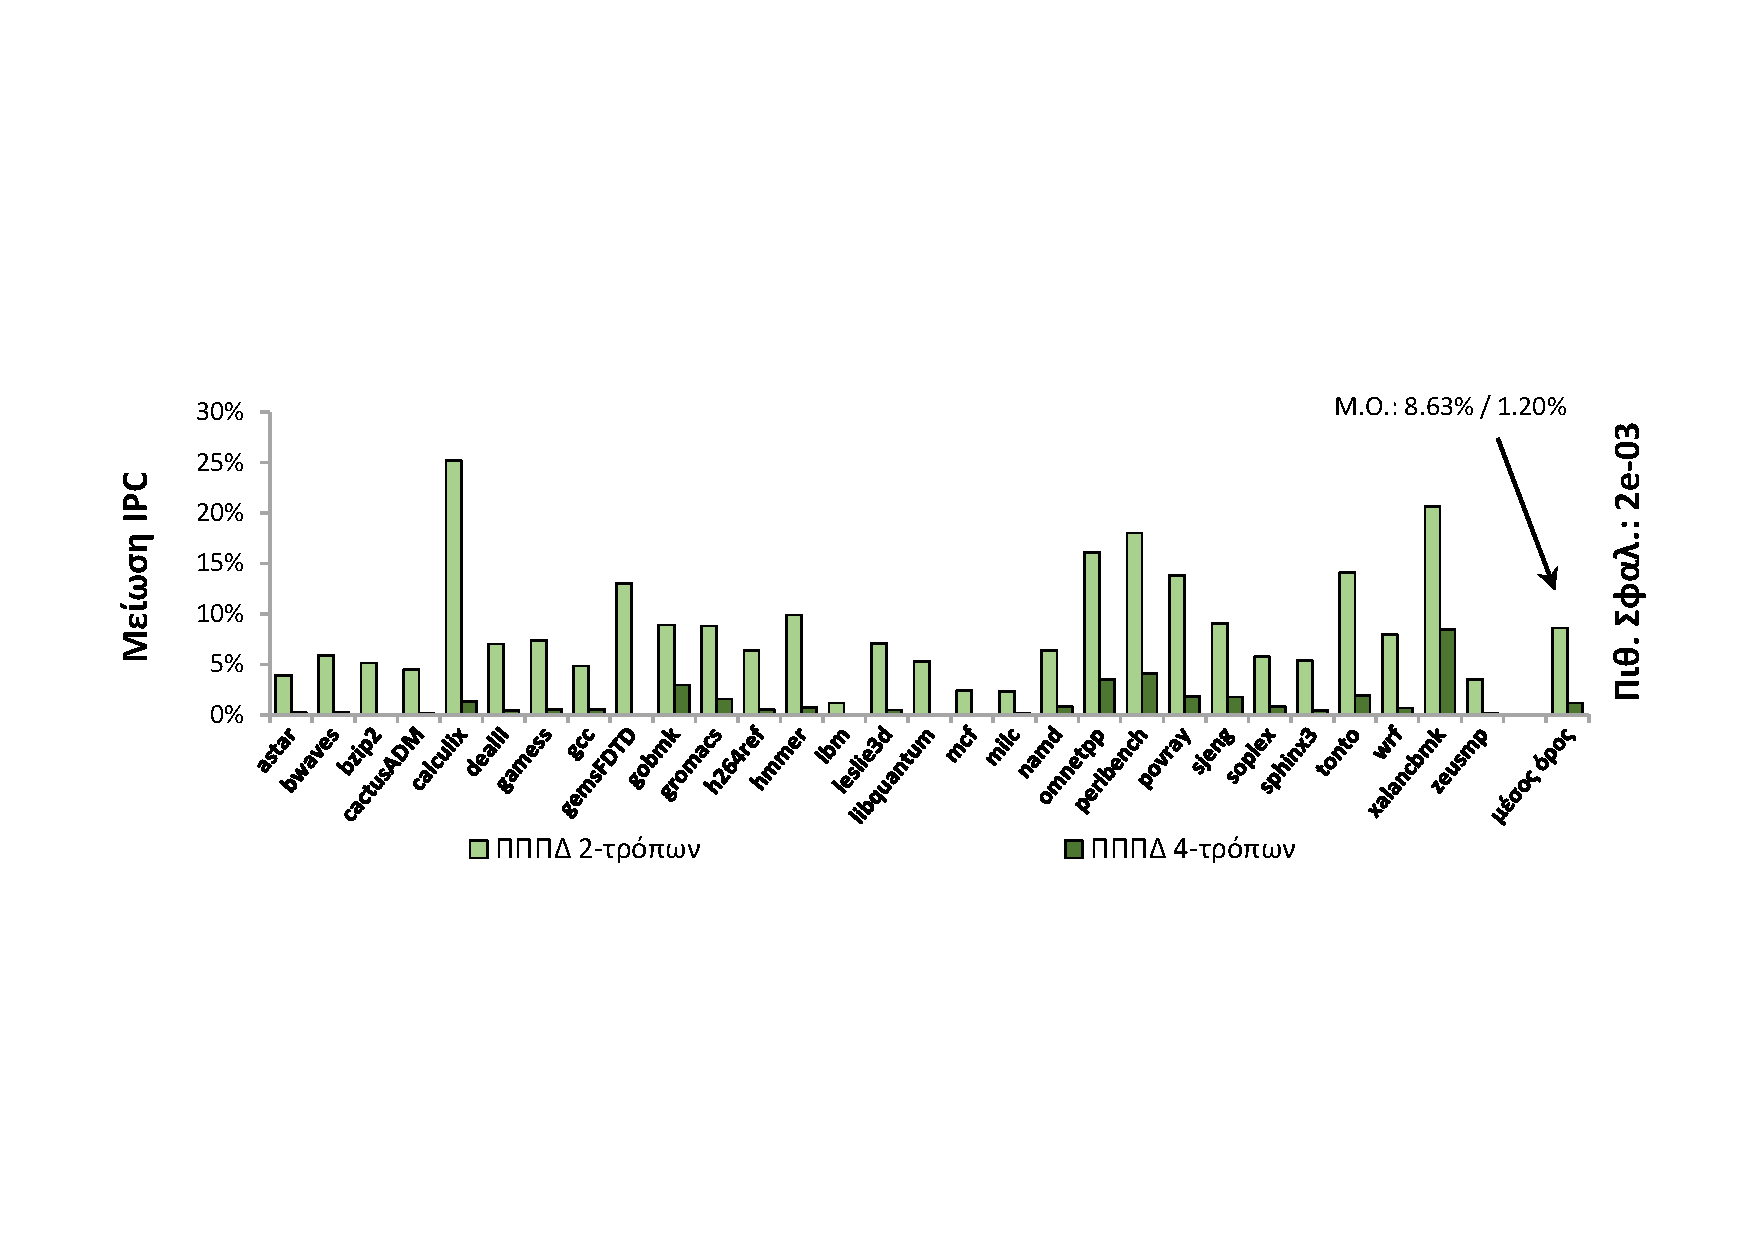
\includegraphics[width=\linewidth, trim=1.9cm 6.4cm 1.8cm 6.6cm, clip=true]{\resultsDIR/chap4_BTB_faulty_ipc_pfail1.pdf}}
        \caption{Πιθανότητα Σφάλματος 1}
        \label{fig:chap4_faulty_pail1_ipc}
    \end{subfigure}
    
    \begin{subfigure}[t]{\textwidth}
        \centering
        \fbox{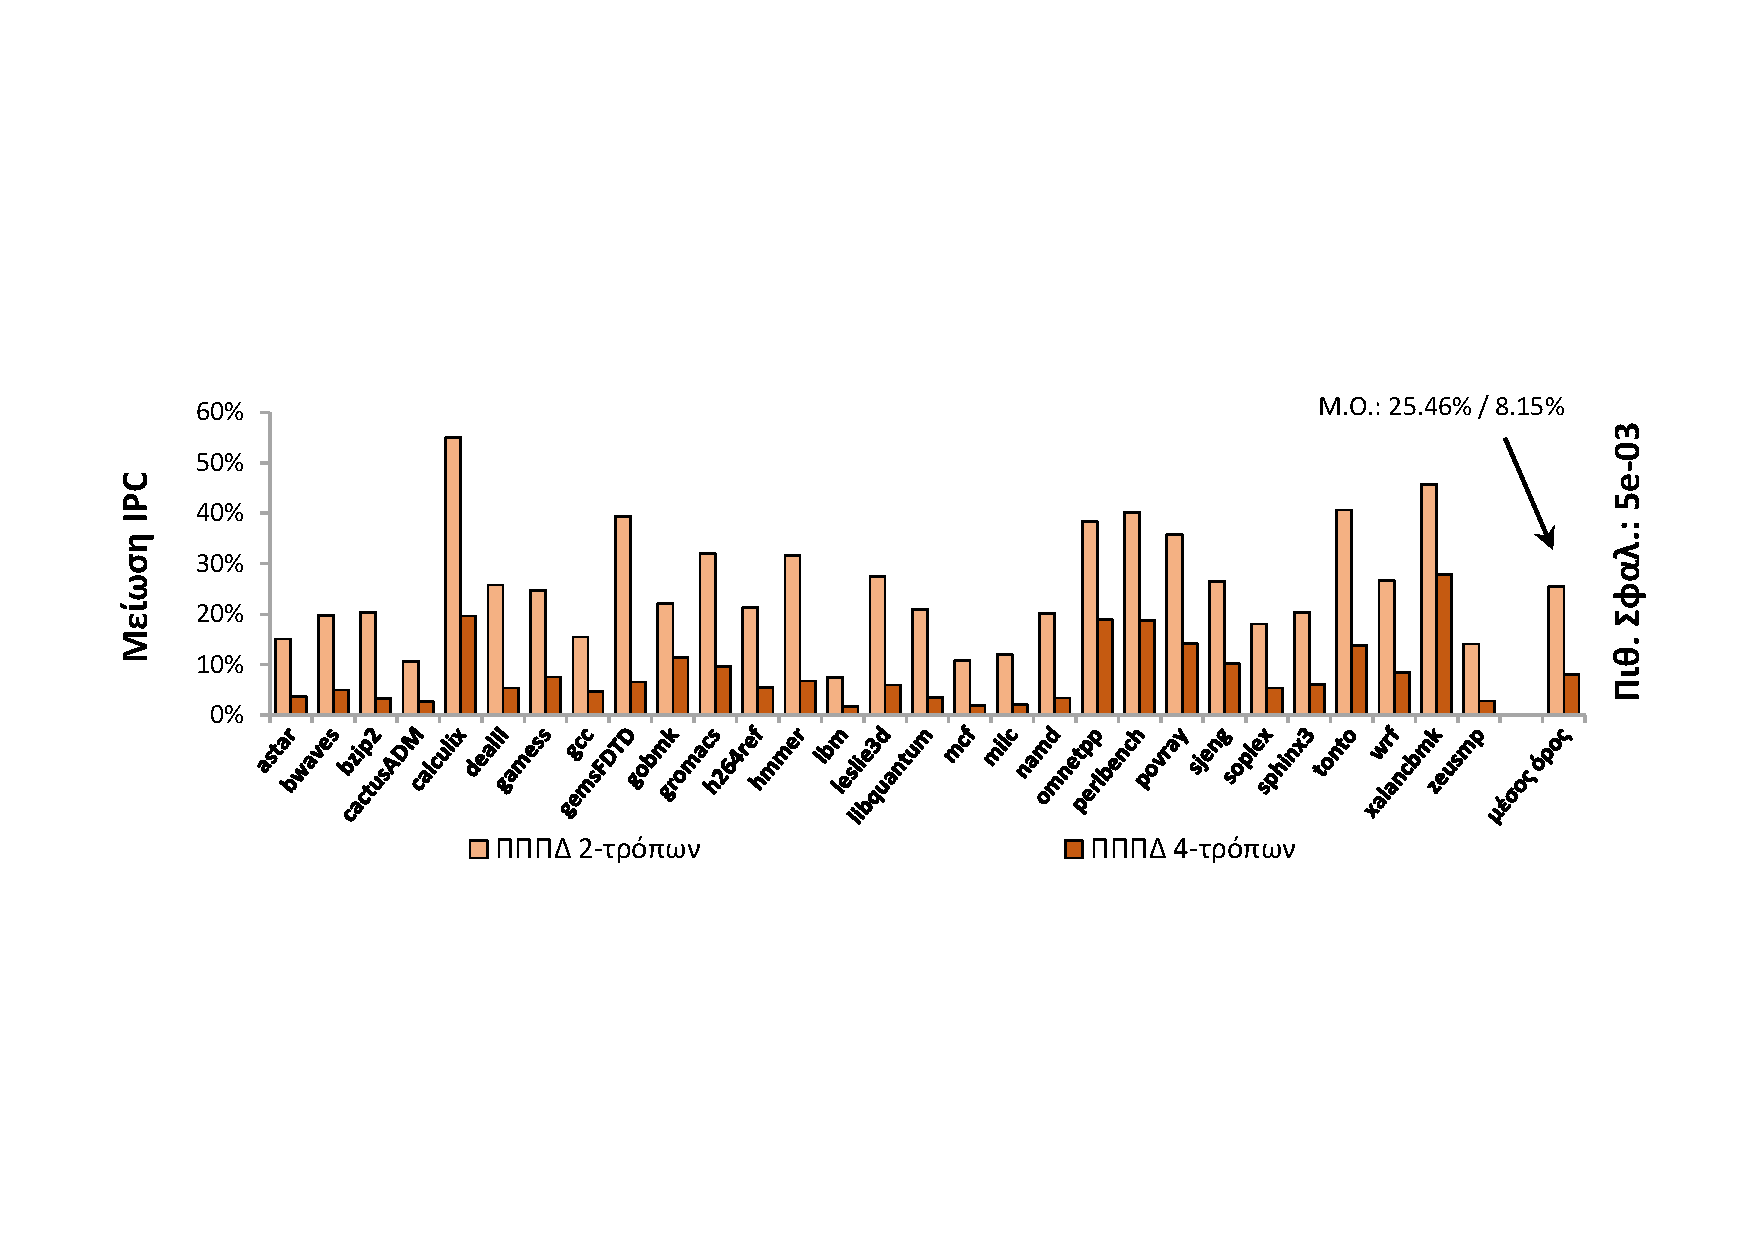
\includegraphics[width=\linewidth, trim=1.9cm 6.4cm 1.8cm 6.6cm, clip=true]{\resultsDIR/chap4_BTB_faulty_ipc_pfail2.pdf}}
        \caption{Πιθανότητα Σφάλματος 2}
        \label{fig:chap4_faulty_pail2_ipc}
    \end{subfigure}
    \caption{Μείωση του ρυθμού ολοκλήρωσης εντολών εξαιτίας της ύπαρξης σφαλμάτων στον Πίνακα Πρόβλεψης Προορισμού Διακλάδωσης, σε σχέση με την περίπτωση εφαρμογής της ονομαστικής τάσης στην ίδια συχνότητα λειτουργίας}
    \label{fig:chap4_faulty_ipc}
\end{figure}

Όπως αναγράφονται και στα αντίστοιχα γραφήματα, το μέγεθος της μείωσης της απόδοσης διαφέρει μεταξύ των πιθανοτήτων και οργανώσεων. Σε μνήμες οργάνωσης 2-τρόπων συνόλου συσχέτισης, στην μελετώμενη πιθανότητα σφάλματος 1 ($\expnum{2}$) η μείωση της απόδοσης φτάνει το 8.63\% κατά μέσο όρο, ενώ στην πιθανότητα σφάλματος 2 ($\expnum{5}$) η μείωση αυτή ξεπερνά το 25\%. Σε μνήμες οργάνωσης 4-τρόπων οι αντίστοιχες μειώσεις κατά μέσο όρο είναι 1.2\% στην πιθανότητα σφάλματος 1, και λίγο πάνω από 8\% στην πιθανότητα σφάλματος 2. Παρόλα αυτά, όπως φαίνεται και στα γραφήματα, υπάρχουν περιπτώσεις μετροπρογραμμάτων όπου η επίπτωση των σφαλμάτων είναι πολύ μεγαλύτερη του μέσου όρου, όπως για παράδειγμα το μετροπρόγραμμα \en{xalancbmk}.

%----------------------------------------------------------%

\section{Μεταβολή της Απόδοσης}
\label{chap4_PerformanceVariation}

Η παρούσα ενότητα συμβάλει στην καλύτερη κατανόησης των περιπτώσεων όπου η μεταβολή της απόδοσης του Πίνακα Πρόβλεψης Προορισμού Διακλάδωσης επιφέρει μεταβολή στην απόδοση του υπερβαθμωτού επεξεργαστή. Η πρώτη υποενότητα επικεντρώνεται στην οργάνωση του Πίνακα Πρόβλεψης Προορισμού Διακλάδωσης (ΠΠΠΔ) και παρουσιάζει την αύξηση της απόδοσης καθώς το μέγεθος και το πλήθος των τρόπων συσχέτισης αυξάνεται, όταν το ολοκληρωμένο λειτουργεί στην ονομαστική τάση. Στη δεύτερη υποενότητα μελετάται πως ο βαθμός παραλληλίας της Κεντρικής Μονάδας Επεξεργασίας (ΚΜΕ) μεταβάλει την επιρροή που έχουν τα σφάλματα του Πίνακα Πρόβλεψης Προορισμού Διακλάδωσης στην απόδοση του συστήματος. Τα αποτελέσματα φανερώνουν εάν και πότε είναι ωφέλιμο να αντιμετωπιστούν τα σφάλματα αυτά.

%----------------------------------------------------------%

\subsection{Οργάνωση ΠΠΠΔ}
\label{chap4_BTBConfigIPC}

\begin{figure}[!b]
    \centering
    \fbox{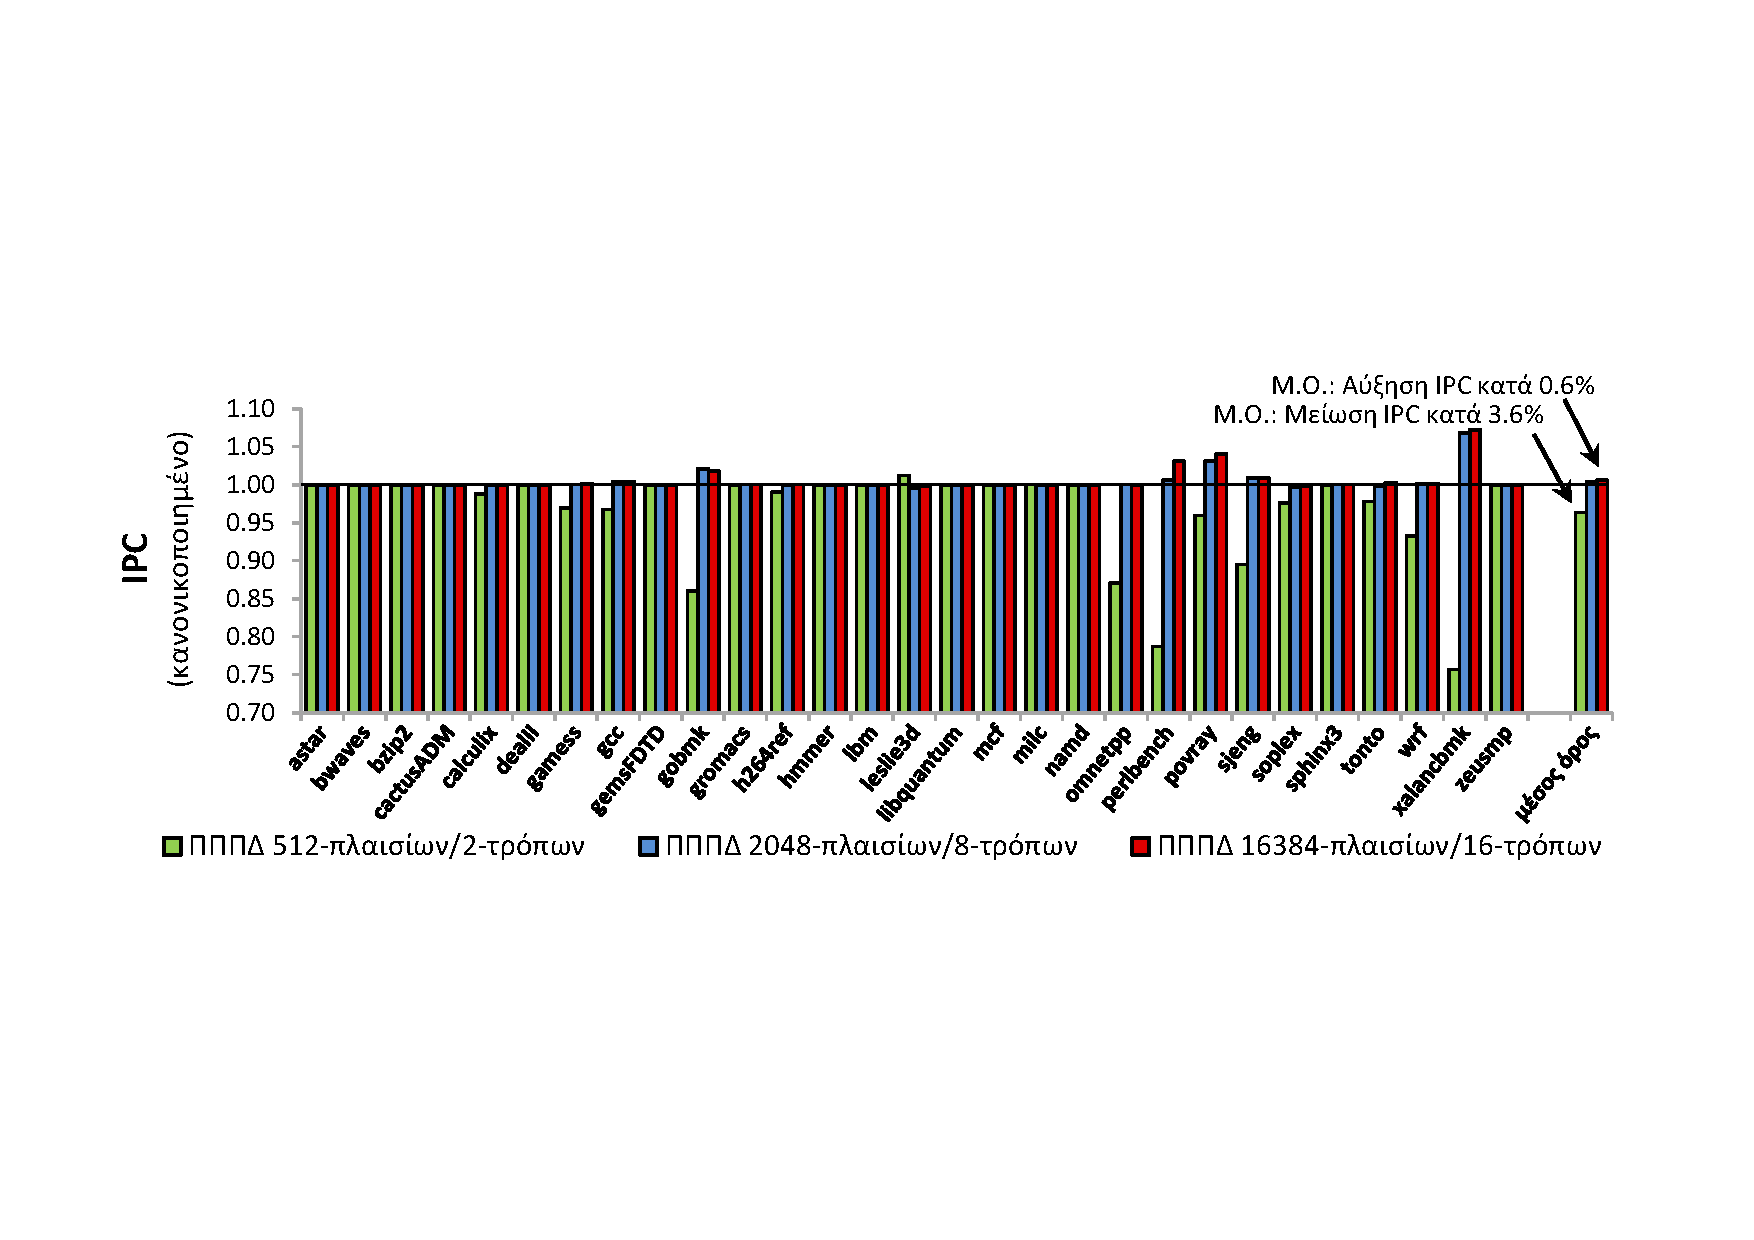
\includegraphics[width=\linewidth, trim=1.9cm 6.4cm 1.8cm 6.3cm, clip=true]{\resultsDIR/chap4_BTB_configs_ipc.pdf}}
    \caption{Ρυθμός ολοκλήρωσης εντολών για διαφορετικές παραμετροποιήσεις του Πίνακα Πρόβλεψης Προορισμού Διακλάδωσης (κανονικοποιημένος ως προς την περίπτωση 2048-πλαισίων/2-τρόπων)}
    \label{fig:chap4_btb_config_performance}
\end{figure}

Στο Σχήμα \ref{fig:chap4_btb_config_performance} παρουσιάζεται η μεταβολή του αριθμού εντολών που ολοκληρώνονται ανά κύκλο (\ipc), με τη μεταβολή του μεγέθους και της οργάνωσης του Πίνακα Πρόβλεψης Προορισμού Διακλάδωσης (ΠΠΠΔ). Τα αποτελέσματα αναφέρονται στην περίπτωση όπου εφαρμόζεται κανονική τάση λειτουργίας και είναι κανονικοποιημένα ως προς την περίπτωση που χρησιμοποιείται Πίνακας Πρόβλεψης Προορισμού Διακλάδωσης 2048 πλαισίων και 2-τρόπων συνόλου συσχέτισης.
\par
Όπως φανερώνεται από το γράφημα του Σχήματος \ref{fig:chap4_btb_config_performance}, η αύξηση του μεγέθους του Πίνακα Πρόβλεψης Προορισμού Διακλάδωσης επηρεάζει ελάχιστα την απόδοση από ένα σημείο κι έπειτα. Συγκεκριμένα, η χρήση πίνακα 512 αντί 2048 πλαισίων (μπάρες πράσινου χρώματος), θα έχει ως αποτέλεσμα τη μείωση του ρυθμού ολοκλήρωσης εντολών κατά 3.6\%, κατά μέσο όρο. Από την άλλη πλευρά, η χρήση ενός πίνακα των 16384 αντί 2048 πλαισίων (μπάρες κόκκινου χρώματος), προσφέρει κατά μέσο όρο λιγότερο από 1\% βελτίωση στο ρυθμού ολοκλήρωσης εντολών.
\par
Μελετώντας τη μεταβολή της απόδοσης με τη μεταβολή του πλήθους τρόπων συσχέτισης, γίνεται αντιληπτό πως η αύξηση του πλήθους πλαισίων ανά σύνολο δεν συνεισφέρει στη βελτίωση της απόδοσης (σχέση μεταξύ πίνακα 2048-πλαισίων/2-τρόπων και 2048-πλαισίων/8-τρόπων). Κατά μέσο όρο όταν χρησιμοποιείται ο πίνακας 2048-πλαισίων/8-τρόπων η βελτίωση είναι μικρότερη από 0.5\% (μπάρες γαλάζιου χρώματος). Ιδιαίτερη μεταβολή στην απόδοση παρουσιάζει το μετροπρόγραμμα \en{xalancbmk}, όπου όταν χρησιμοποιηθεί πίνακας του ίδιο μεγέθους (2048-πλαισίων) αλλά τετραπλάσιας συσχέτισης (8-τρόπων αντί για 2-τρόπων), παρουσιάζει βελτίωση μεγαλύτερη από 7\%. Αντίστοιχα, όταν το μέγεθος και το πλήθος των τρόπων συσχέτισης μειώνονται (από πίνακα 2048-πλαισίων/2-τρόπων σε πίνακα 512-πλαισίων/2-τρόπων), η μείωση της απόδοσης ξεπερνά το 24\%.
\par
Επομένως, για τη εκτέλεσης μίας μέσης περίπτωσης προγράμματος είναι προτιμότερο κατά το σχεδιασμό του υπερβαθμωτού επεξεργαστή να χρησιμοποιείται Πίνακας Πρόβλεψης Προορισμού Διακλάδωσης 2048-πλαισίων και μικρού σχετικά πλήθους πλαισίων ανά σύνολο, μειώνοντας έτσι την κατανάλωση σε σχέση με ένα πίνακα μεγαλύτερου μεγέθους και πλήθους πλαισίων ανά σύνολο.

%----------------------------------------------------------%

\subsection{Παραλληλία ΚΜΕ και Σφάλματα ΠΠΠΔ}
\label{chap4_CoreConfigIPC}

Στο Σχήμα \ref{fig:chap4_core_config_performance} παρουσιάζονται τα αποτελέσματα τεσσάρων διαφορετικών παραμετροποιήσεων του εξομοιούμενου επεξεργαστή, όταν η τάση λειτουργίας μειώνεται με αποτέλεσμα να εμφανίζονται ελαττωματικά πλαίσια στον Πίνακα Πρόβλεψης Προορισμού Διακλάδωσης. Συγκεκριμένα, τα αποτελέσματα αναφέρονται στην τάση λειτουργίας που αντιστοιχεί σε πιθανότητα σφάλματος $\expnum{2}$, όπου σύμφωνα με την ανάλυση της Ενότητας \ref{chap4_BranchTargetBufferFaults} το 20\% σχεδόν των πλαισίων είναι απενεργοποιημένα εξαιτίας των σφαλμάτων. Ξεκινώντας από έναν επεξεργαστή βαθμού παραλληλίας 1 (προσκόμιση, αποκωδικοποίηση, εκτέλεσης και ολοκλήρωσης μίας εντολής σε κάθε κύκλο), απεικονίζεται η μεταβολή της απόδοσης εξαιτίας της ύπαρξης σφαλμάτων στη Μονάδα Δυναμικής Πρόβλεψης Διακλαδώσεων, καθώς ο βαθμός παραλληλίας διπλασιάζεται (προσκόμιση, αποκωδικοποίηση, εκτέλεση και ολοκλήρωσης διπλάσιων εντολών σε κάθε κύκλο). Σε αυτό το σημείο πρέπει να επισημανθεί πως ο επεξεργαστής βαθμού παραλληλίας 1 δεν ισοδυναμεί με έναν σε-σειρά επεξεργαστή, καθώς οι εντολές που προσκομίζονται μπορούν να εκτελούνται με διαφορετική σειρά και να ολοκληρώνονται με τη σωστή.

\begin{figure}[t]
    \centering
    \fbox{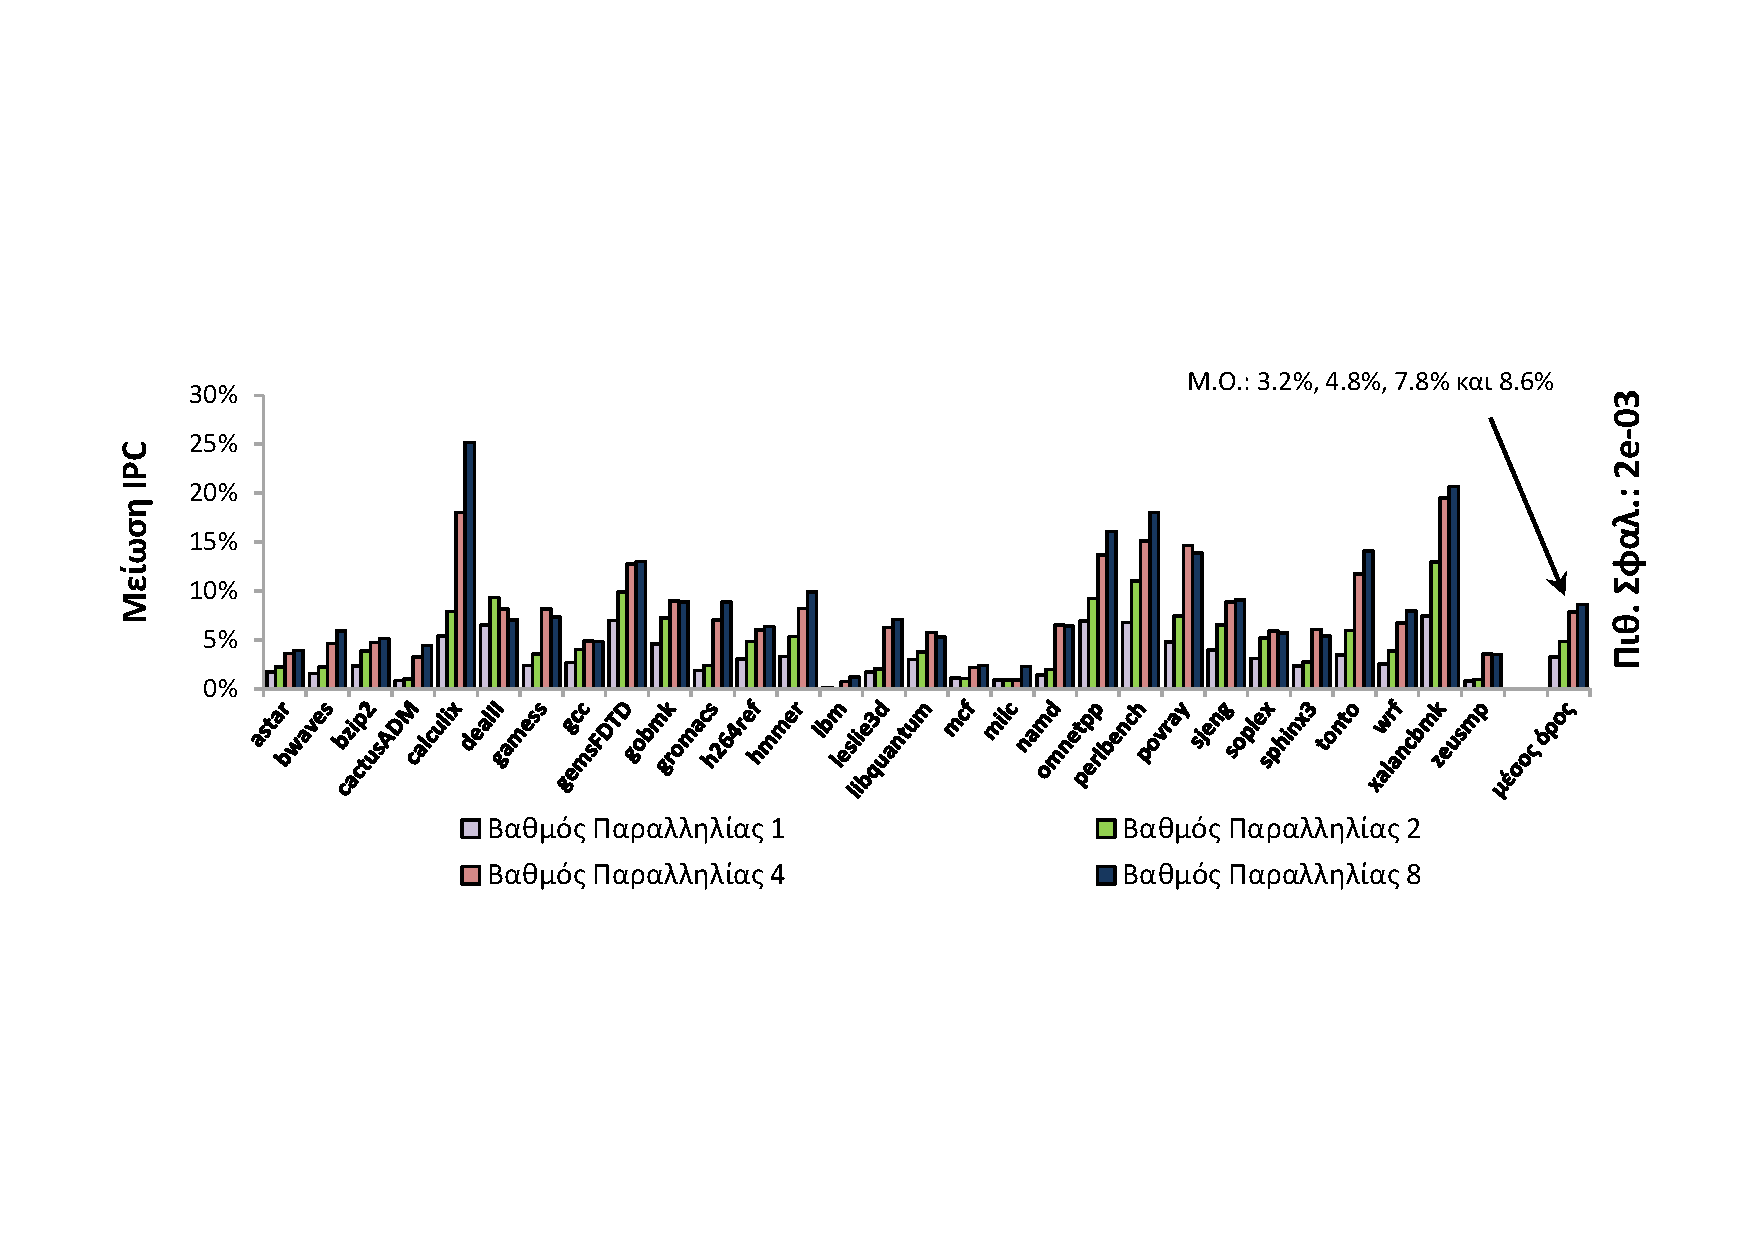
\includegraphics[width=\linewidth, trim=1.9cm 6.0cm 1.8cm 6.2cm, clip=true]{\resultsDIR/chap4_CORE_configs_ipc.pdf}}
    \caption{Μείωση του ρυθμού ολοκλήρωσης εντολών όταν υπάρχουν ελαττωματικά πλαίσια στον Πίνακα Πρόβλεψης Προορισμού Διακλάδωσης, για τέσσερα διαφορετικά μοντέλα εξομοιούμενων επεξεργαστών}
    \label{fig:chap4_core_config_performance}
\end{figure}

Ένα πολύ σημαντικό συμπέρασμα που μπορεί να εξαχθεί από το γράφημα του Σχήματος \ref{fig:chap4_core_config_performance}, είναι πως η επιρροή των σφαλμάτων της Μονάδας Δυναμικής Πρόβλεψης Διακλαδώσεων στην απόδοση γίνεται εντονότερη καθώς ο βαθμός παραλληλίας αυξάνεται. Συγκεκριμένα, στον επεξεργαστή βαθμού παραλληλίας 1 η μείωση της απόδοσης όταν στον Πίνακα Πρόβλεψης Προορισμού Διακλάδωσης υπάρχουν ελαττωματικά πλαίσια, είναι κατά μέσο όρο μόλις 3.2\%. Το ποσοστό αυτό ανεβαίνει σε 4.8\%, 7.8\% και 8.6\% με την αύξηση του βαθμού παραλληλίας αντίστοιχα. Το γεγονός αυτό είναι αναμενόμενο καθώς η προσκόμιση περισσότερων εντολών σε κάθε κύκλο ρολογιού συνεπάγεται και αύξηση των περιττών εντολών που θα προσκομιστούν στο Μηχανισμό Μερικώς Επικαλυπτόμενων Λειτουργιών, σε περίπτωση που υπάρξει λανθασμένη πρόβλεψη εντολής διακλάδωσης. Αυτό θα έχει ώς συνέπεια την εκτέλεση εντολών οι οποίες θα καταναλώσουν πολύτιμο χρόνο και ενέργεια έως ότου ανιχνευθεί η λανθασμένη πρόβλεψη, χωρίς να χρησιμοποιηθούν τελικώς τα αποτελέσματά τους. Για το λόγο αυτό δείχνει απαραίτητο να εξασφαλίζεται η κατά το δυνατόν αποδοτικότερη λειτουργία της Μονάδας Δυναμικής Πρόβλεψης Διακλαδώσεων σε επεξεργαστές που παρουσιάζουν αυξημένο βαθμό παραλληλίας.
\par
Οι τέσσερις περιπτώσεις διαφορετικών παραμέτρων που χρησιμοποιήθηκαν παρουσιάζονται στον Πίνακα \ref{tab:chap4_CoreConfigs}. Αναλυτικά δεδομένα για τα υπόλοιπα στοιχεία του μηχανισμού αναγράφονται στον Πίνακα \ref{tab:chap6_gem5parameters}, όπου περιγράφεται το γενικό μοντέλο που χρησιμοποιήθηκε κατά τη διαδικασίας της αξιολόγηση.

\begin{table}[!b]
    \centering
    %\begin{tabularx}{\textwidth}{!{\vrule width 4\arrayrulewidth} >{\centering\arraybackslash}X | >{\centering\arraybackslash}X !{\vrule width 4\arrayrulewidth}}
    \begin{tabularx}{\textwidth}{ >{\centering\arraybackslash}X >{\centering\arraybackslash}X }
    \Xhline{4\arrayrulewidth}
        \multirow{2}{*}{\textbf{Μοντέλο Εξομοίωσης}} & 
        \multirow{2}{\linewidth}{\centering \textbf{Παράμετροι (\en{Width/ROB/IQ/LQ/SQ/Registers})}} \\
        &    \\
        \Xhline{4\arrayrulewidth}
        {ΚΜΕ Βαθμού Παραλληλίας 1} & {1/32/16/16/16/64} \\
        %\hline
        {ΚΜΕ Βαθμού Παραλληλίας 2} & {2/64/32/32/32/64} \\
        %\hline
        {ΚΜΕ Βαθμού Παραλληλίας 4} & {4/128/64/64/64/128} \\
        %\hline
        {ΚΜΕ Βαθμού Παραλληλίας 8} & {8/256/256/128/128/128} \\
        \Xhline{4\arrayrulewidth}
    \end{tabularx}
    \caption{Παραμετροποιήσεις της Κεντρικής Μονάδας Επεξεργασίας}
    \label{tab:chap4_CoreConfigs}
\end{table}

%----------------------------------------------------------%

\section{Συμπεράσματα}
\label{chap4_FaultsAnalysisConclusions}

Παρότι στην Υποενότητα \ref{chap4_BTBConfigIPC} αναφέρθηκε πως η απόδοσης δεν επηρεάζεται αισθητά από το μέγεθος και την οργάνωση του Πίνακα Πρόβλεψης Προορισμού Διακλάδωσης, στην ανάλυση της Υποενότητας \ref{chap4_BranchTargetBufferFaults} παρουσιάζεται μία σημαντική πτώση του ρυθμού ολοκλήρωσης εντολών σε ορισμένες περιπτώσεις. Η αιτίας αυτής της πτώσης της απόδοσης είναι η εμφάνιση πλήρως ελαττωματικών συνόλων. Η αδυναμία αποθήκευσης πληροφορίας για ένα πλήθος εντολών διακλάδωσης θα έχει ώς συνέπεια την υποχρεωτική αναμονή (αδυναμία προσκόμισης νέων εντολών) έως τον υπολογισμό των αντίστοιχων διευθύνσεων προορισμού. Το κατά πόσο επηρεάζει ένα πλήρως ελαττωματικό σύνολο ένα εκτελούμενο πρόγραμμα εξαρτάται από τη διεύθυνση των εντολών διακλάδωσης καθώς, όπως αναφέρθηκε και στην Ενότητα \ref{chap2_BranchTargetBuffer}, η διευθυνσιοδότηση του συνόλου γίνεται από ένα τμήμα της διεύθυνσης εντολής. Επομένως, σε ορισμένες περιπτώσεις η επίδρασή των πλήρως ελαττωματικών συνόλων ενός συγκεκριμένου πίνακα στο χρόνο εκτέλεσης ενός προγράμματος μπορεί να είναι πολύ σημαντική, ενώ σε άλλες όχι.
\par
Γίνεται λοιπόν σαφές πως η ανάπτυξη κατάλληλης τεχνικής για τον περιορισμό των πλήρως ελαττωματικών συνόλων του Πίνακα Πρόβλεψης Προορισμού Διακλάδωσης θα περιόριζε σε μεγάλο βαθμό την αύξηση του χρόνου εκτέλεσης λόγω της εμφάνισης σφαλμάτων στη Μονάδα Δυναμικής Πρόβλεψης Διακλαδώσεων. Στην παρούσα μελέτη γίνεται η πρόταση μίας τέτοιας τεχνικής, η οποία είναι σε θέση να επιφέρει το επιθυμητό αποτέλεσμα σε μεγάλο βαθμό με το ελάχιστο δυνατό κόστος. Τόσο η υλοποίηση της προτεινόμενη τεχνικής όσο και τα αποτελέσματά της παρουσιάζονται στα ακόλουθα κεφάλαια.

%----------------------------------------------------------%
